\chapter{Semantic News Map Application}
\label{chap:semnews-app}

This chapter will present the end user web application which will visualise the already processed news in various interesting ways. Its goal is to allow you to "read" news in an entirely different way. Usually in articles and almost any other forms of text, the relevant and important information consists in probably less than half the whole text. Harnessing the power of semantics as described in \textit{Chapter \ref{chap:news-pipeline}} with presenting a whole processing pipeline for extracting meaningful information from news data, we now possess an extremely powerful asset extracted in an automated way. The next step is how to present this powerful asset to the user in a unique, effective and interesting way. 

\section{Main Functionalities}
The \textit{Semantic News Map} application consists of a set of visualisations that present the relevant content of a news article or a group of news articles by doing aggregations on the already extracted metadata through SPARQL queries against a GraphDB\textsuperscript{TM} repository with all needed data imported. There are two main types of visualisations: 
\begin{itemize}
    \item Word Cloud
    \item Geographic Heat Map
\end{itemize}
The are a few different versions of word clouds that present data based on different criteria:
\begin{enumerate}
    \item \textbf{Direct popularity} of the concepts based on mentions count in the news and degree of importance of these news.
    \item \textbf{Relative popularity} - where the popularity within the current day is normalized against the popularity within the last year.
    \item Concepts that are \textbf{"hidden champions"} - entities that have an indirect relationship to the currently most popular ones.
    \item Combination of \textbf{"hidden champions"} and \textbf{relative popularity}. 
\end{enumerate}
The geographic heat map has two main functionalities:
\begin{enumerate}
    \item Colors all world countries with different degrees of color intensity according to a specified color scale, based on the number of news in which they are mentioned and displays the news count of each when hovering with the mouse over them.
    \item Presents the list of news mentioning a specific county in a side panel when clicking on it.
\end{enumerate}
\newpage

\begin{figure*}[ht!]
    \centering
    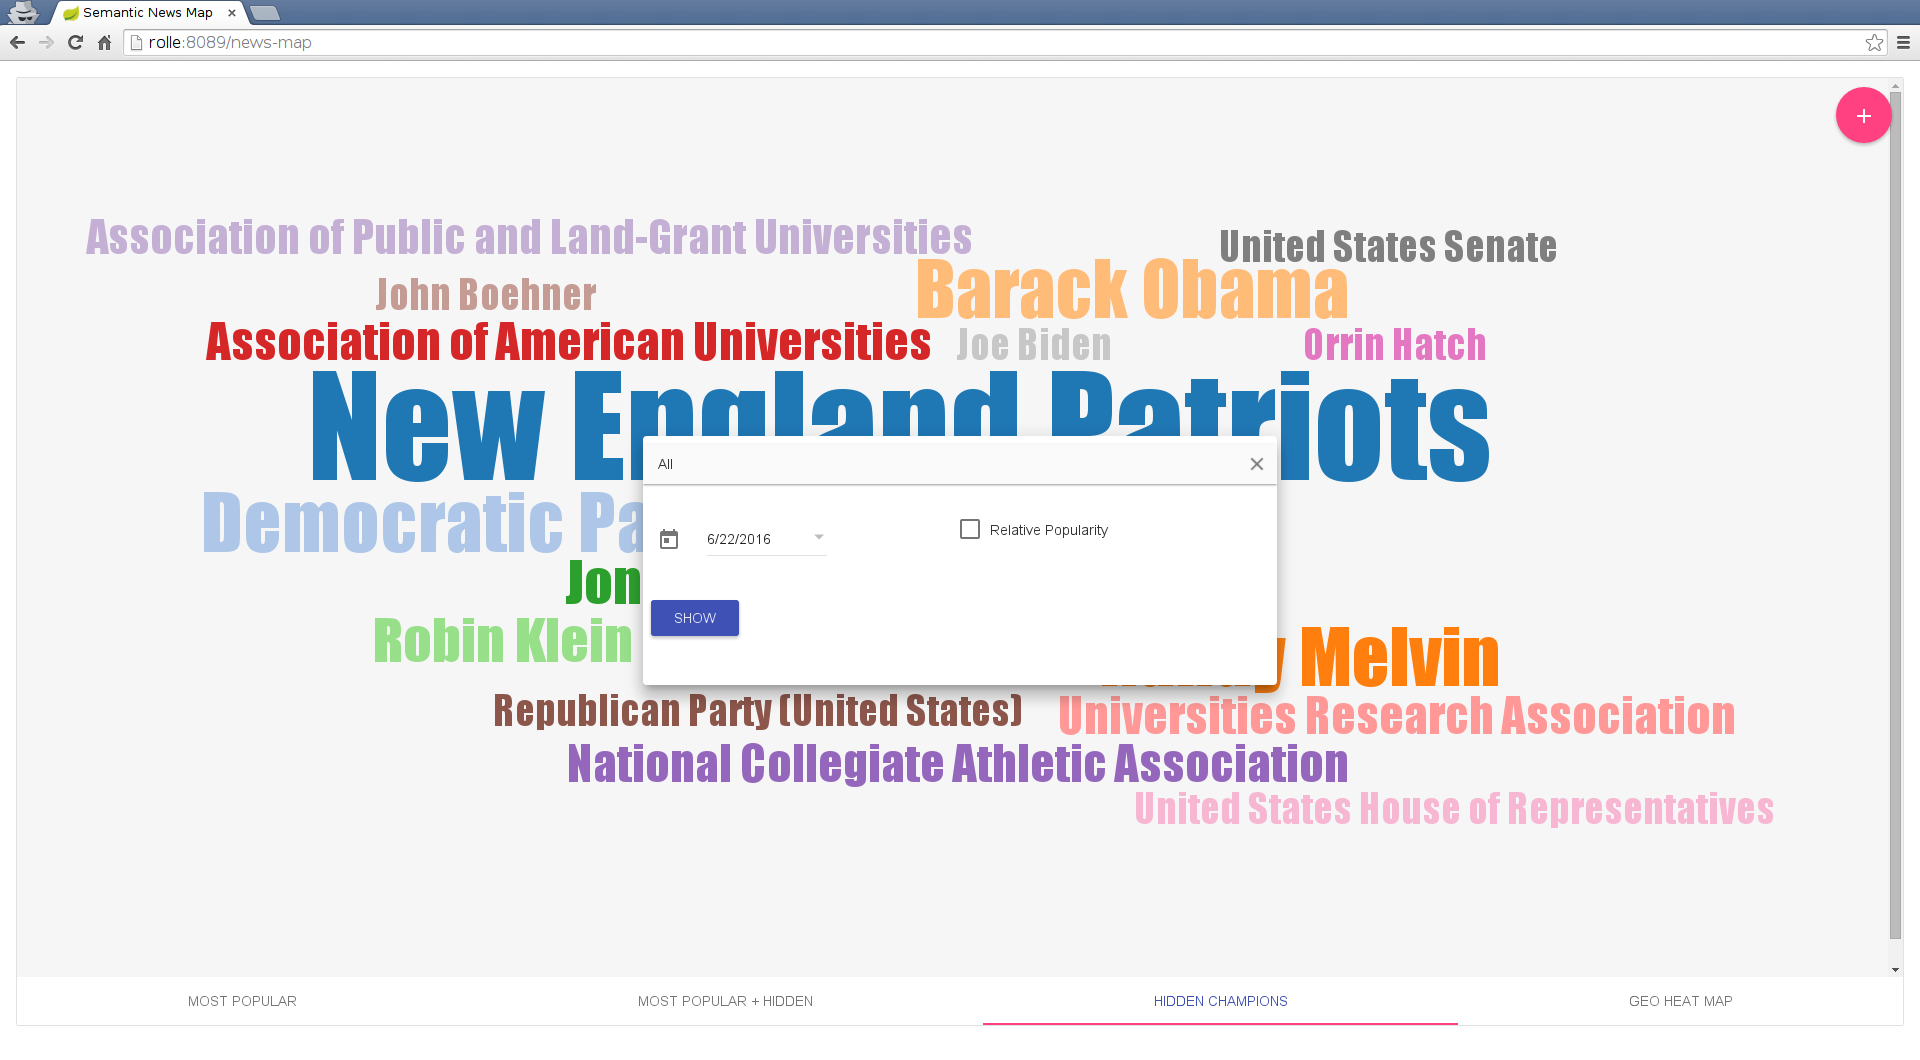
\includegraphics[width=\linewidth]{search-dialog}
    \caption{Hidden Champions criterion word cloud visualisation}
    \label{fig:search-dialog}
\end{figure*}

\begin{figure}[h!]
    \centering
    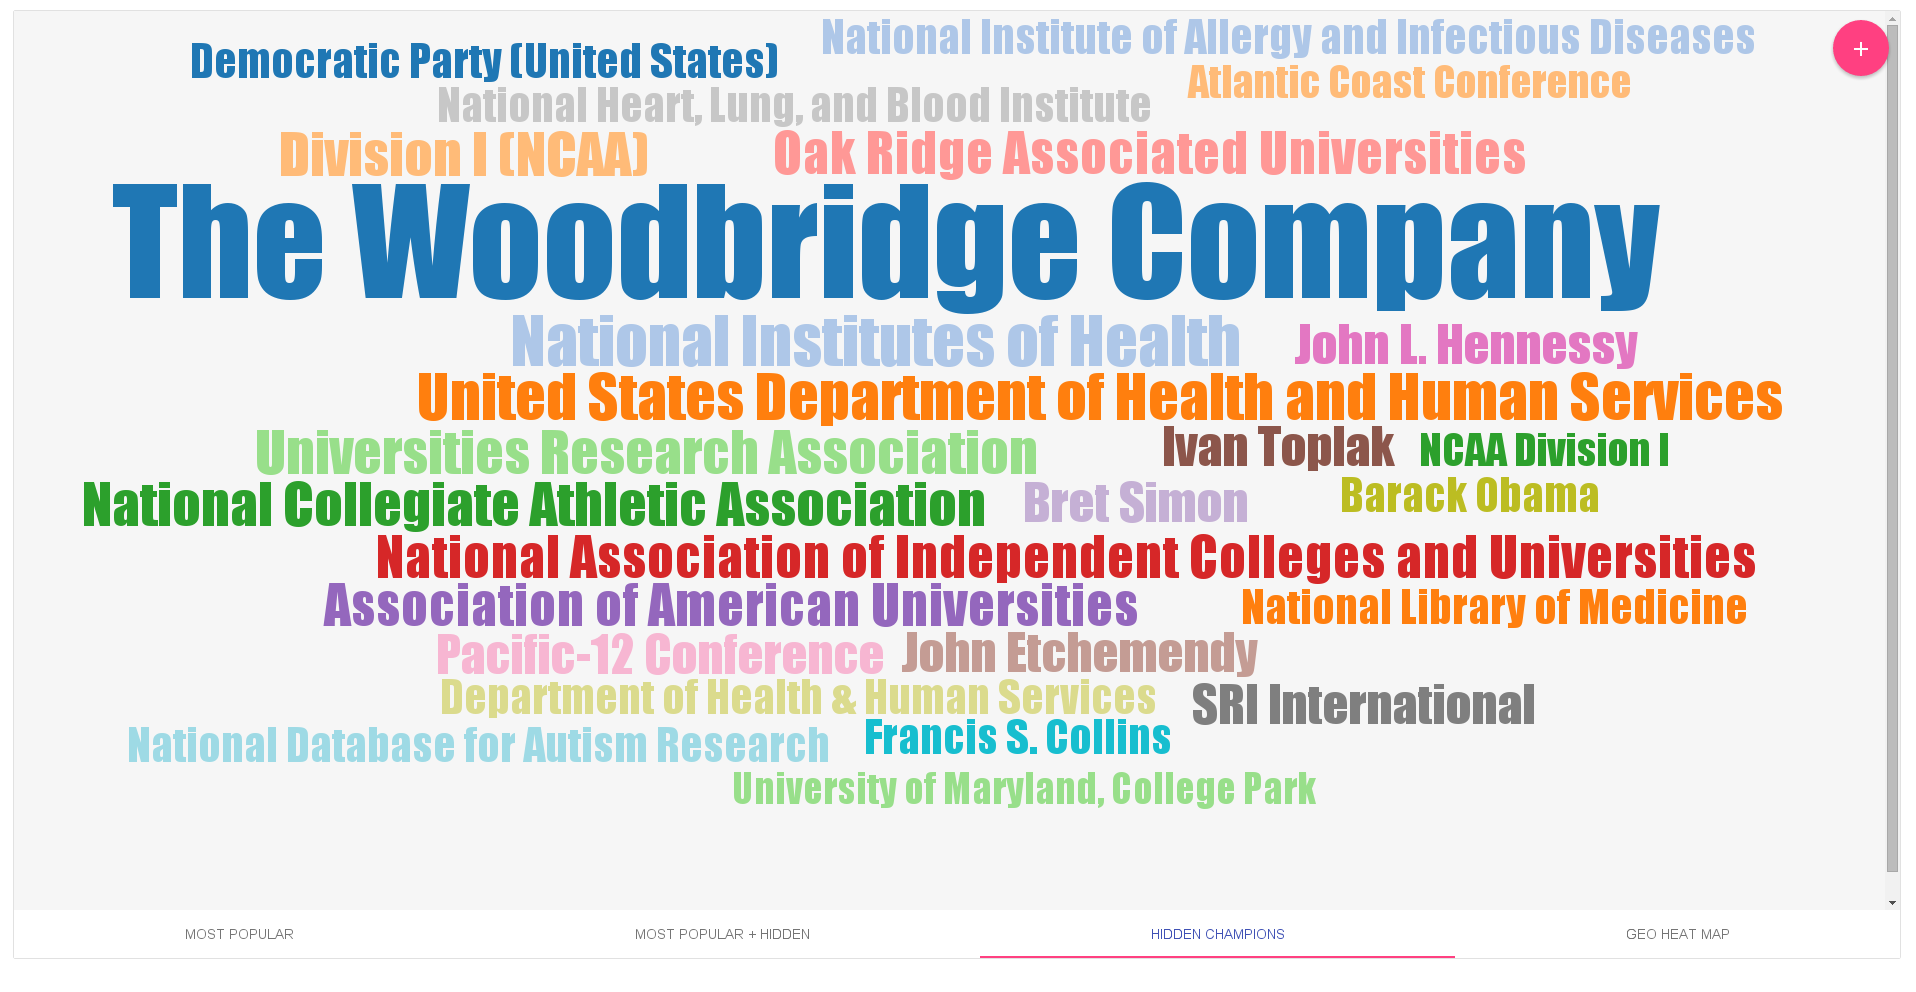
\includegraphics[width=\linewidth]{word-cloud}
    \caption{Hidden Champions criterion word cloud visualisation}
    \label{fig:word-cloud-hidden-champions}
\end{figure}

\begin{figure}[h!]
    \centering
    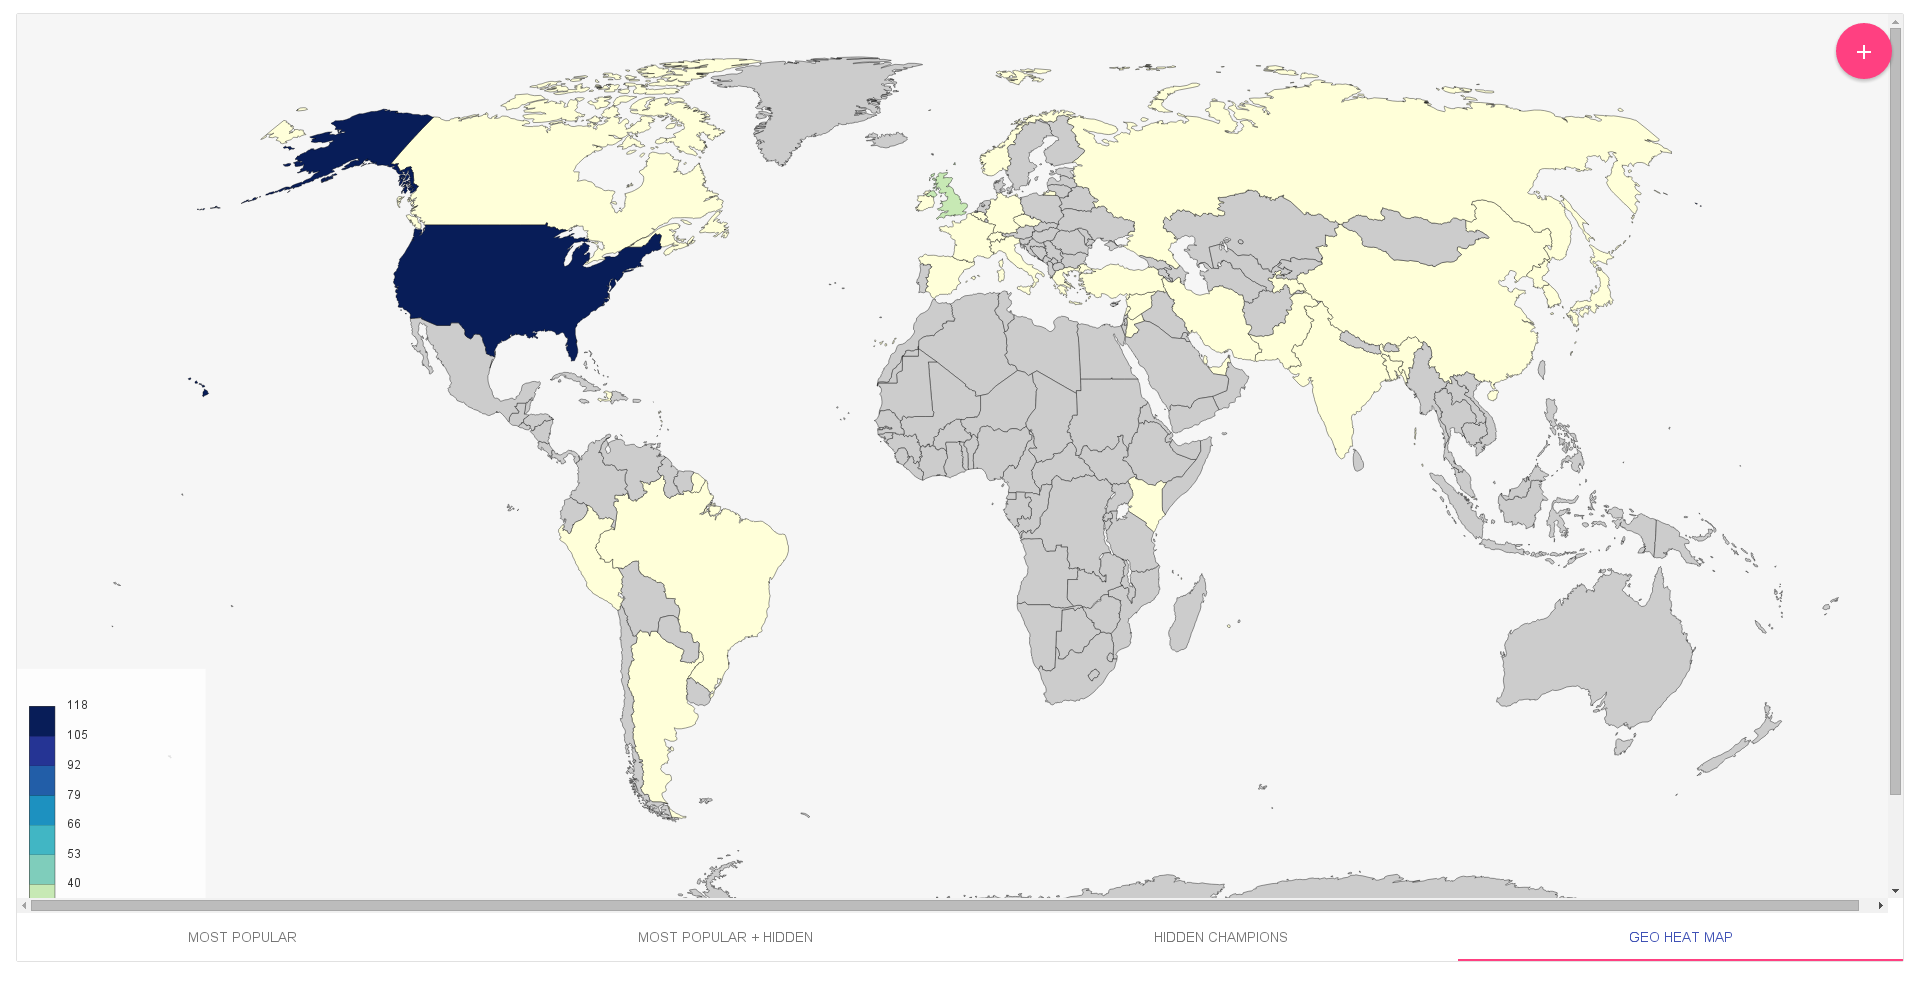
\includegraphics[width=\linewidth]{geoheat-map}
    \caption{Geographic heat map}
    \label{fig:geoheat-map}
\end{figure}

\begin{figure}[h!]
    \centering
    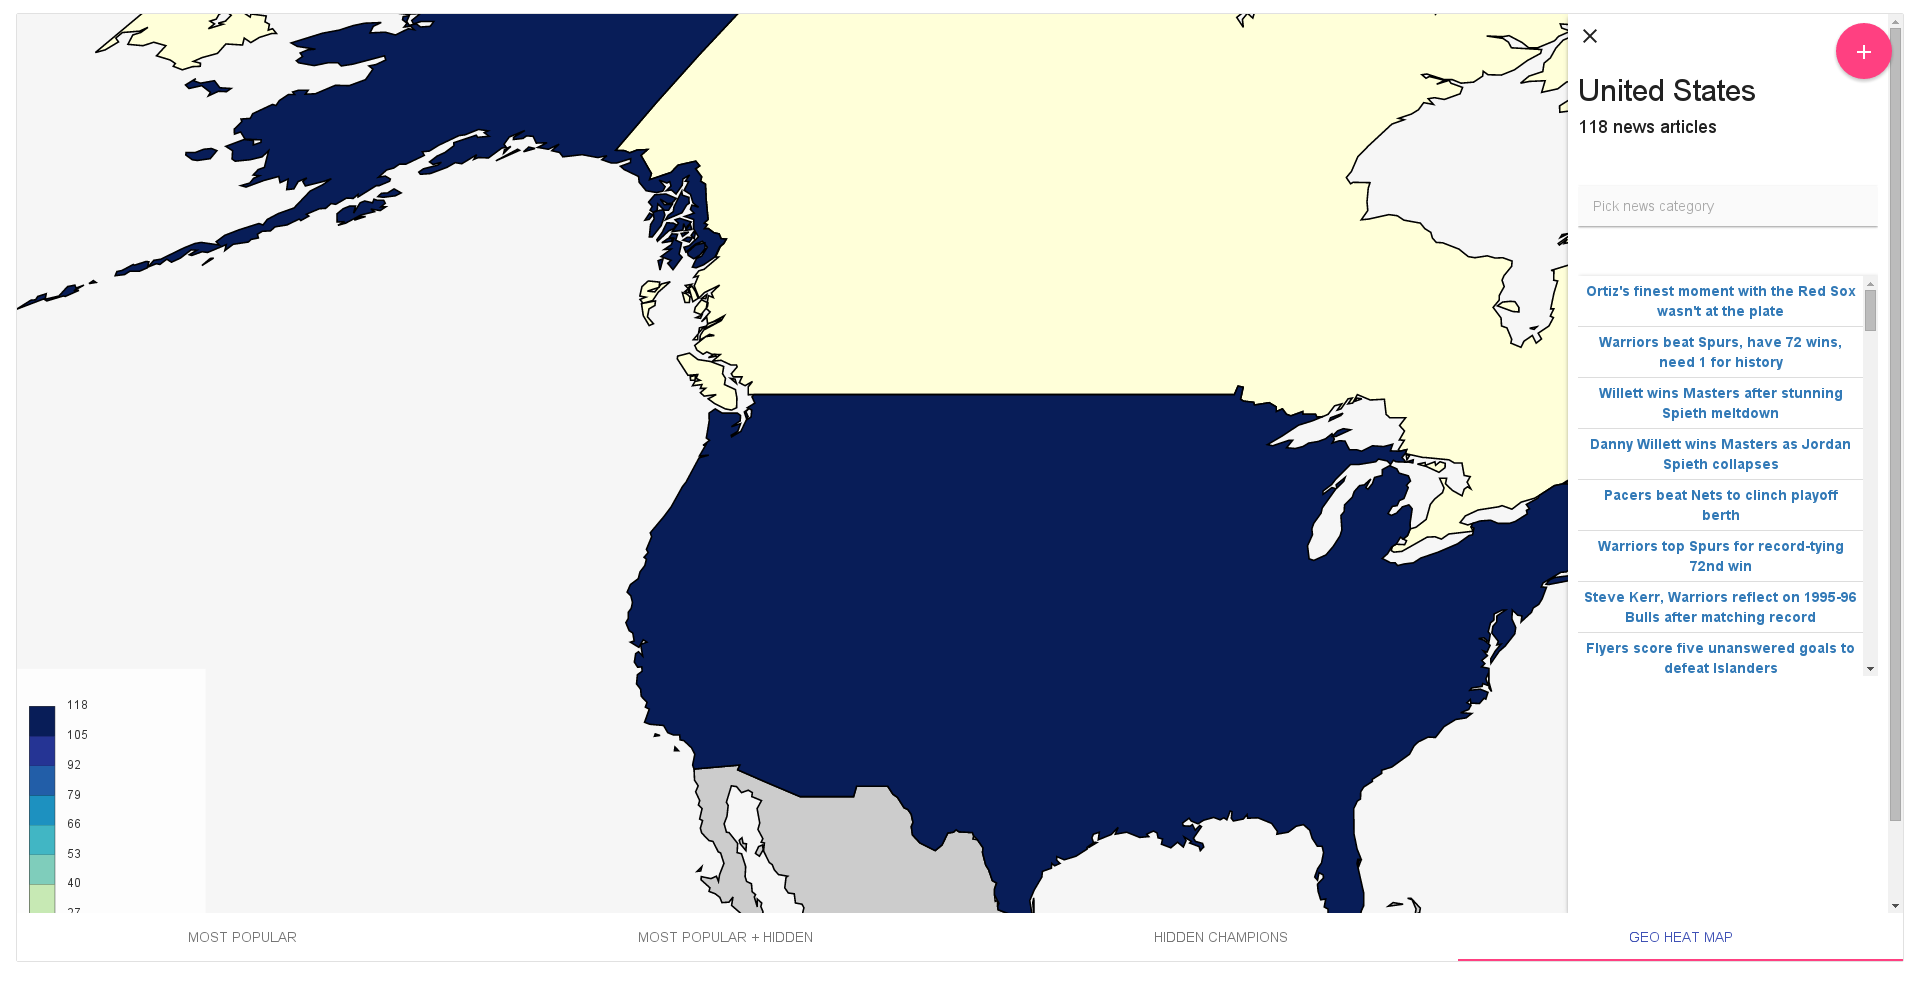
\includegraphics[width=\linewidth]{zoomed-geoheat-map}
    \caption{News mentioning USA and heat map zoomed on USA}
    \label{fig:zoomed-geoheat-map}
\end{figure}

\begin{figure}[h!]
    \centering
    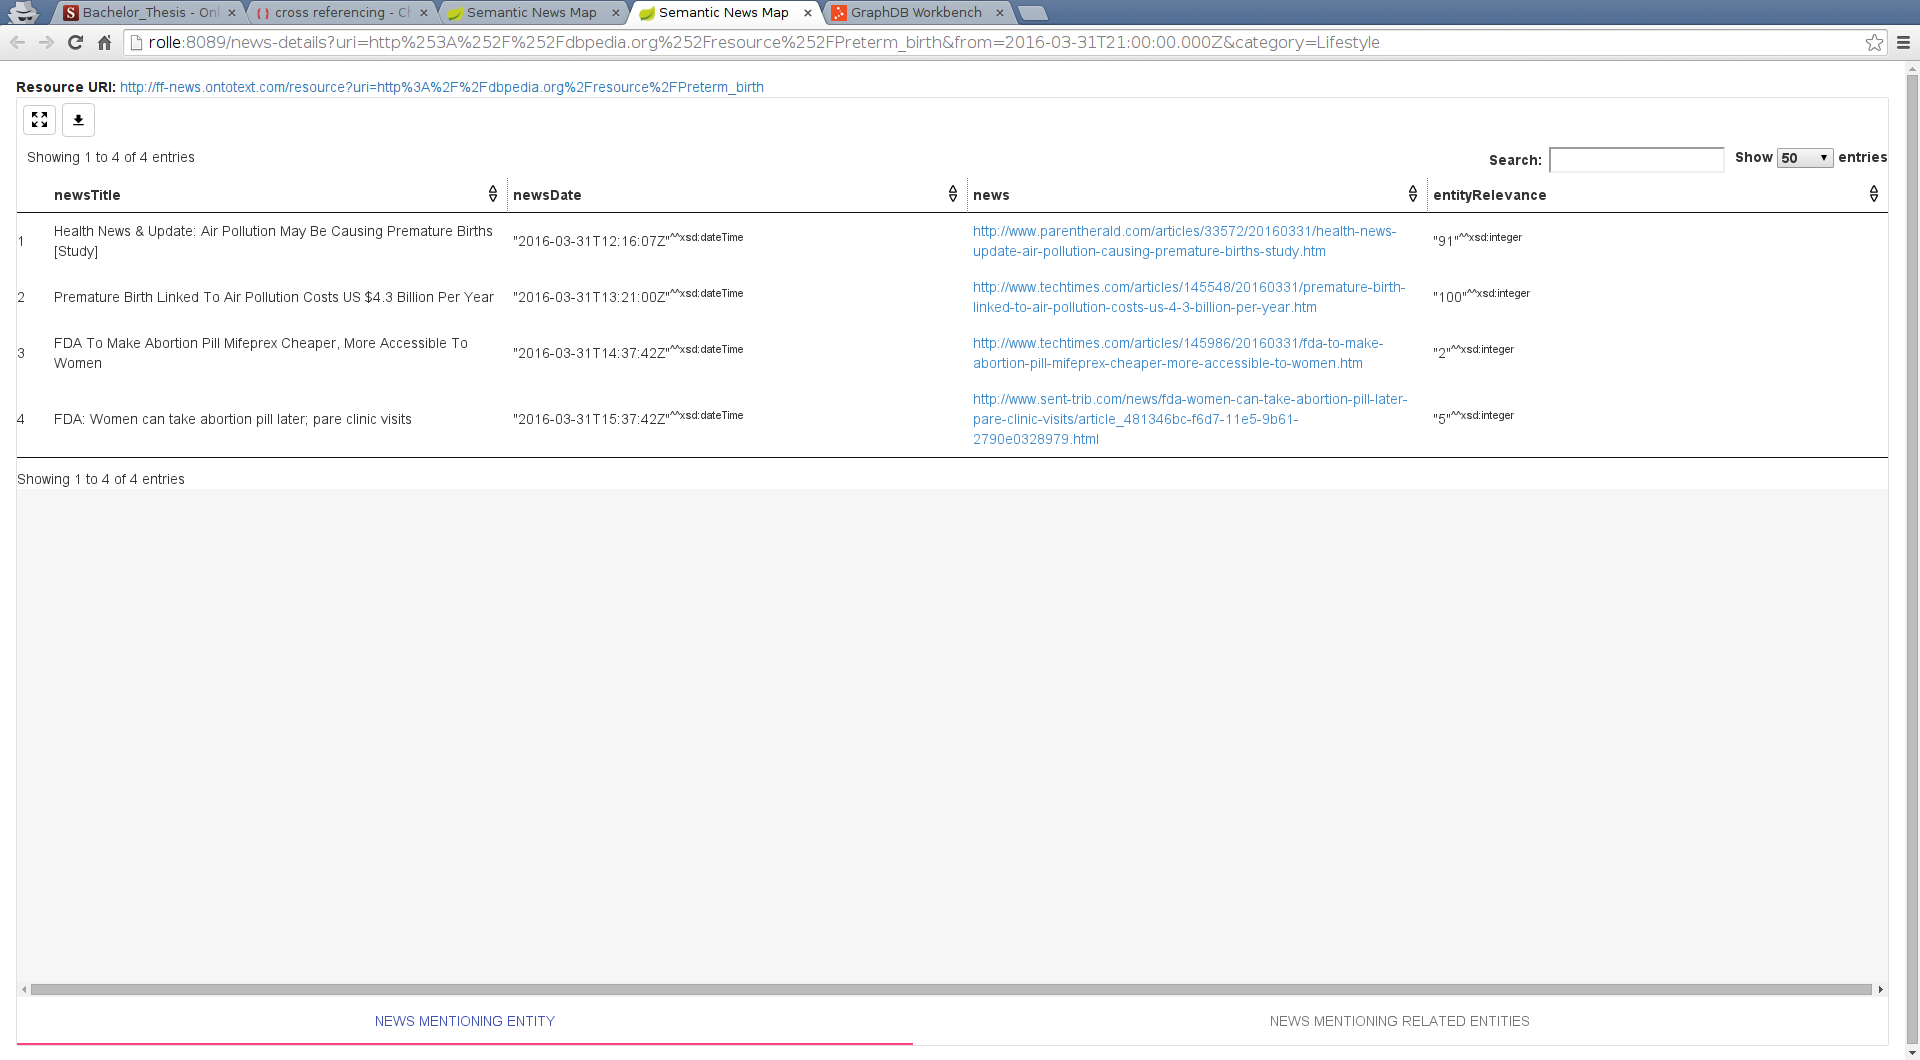
\includegraphics[width=\linewidth]{news-mentioning-entity}
    \caption{News mentioning entity view}
    \label{fig:news-mentioning-entity}
\end{figure}

\begin{figure}[h!]
    \centering
    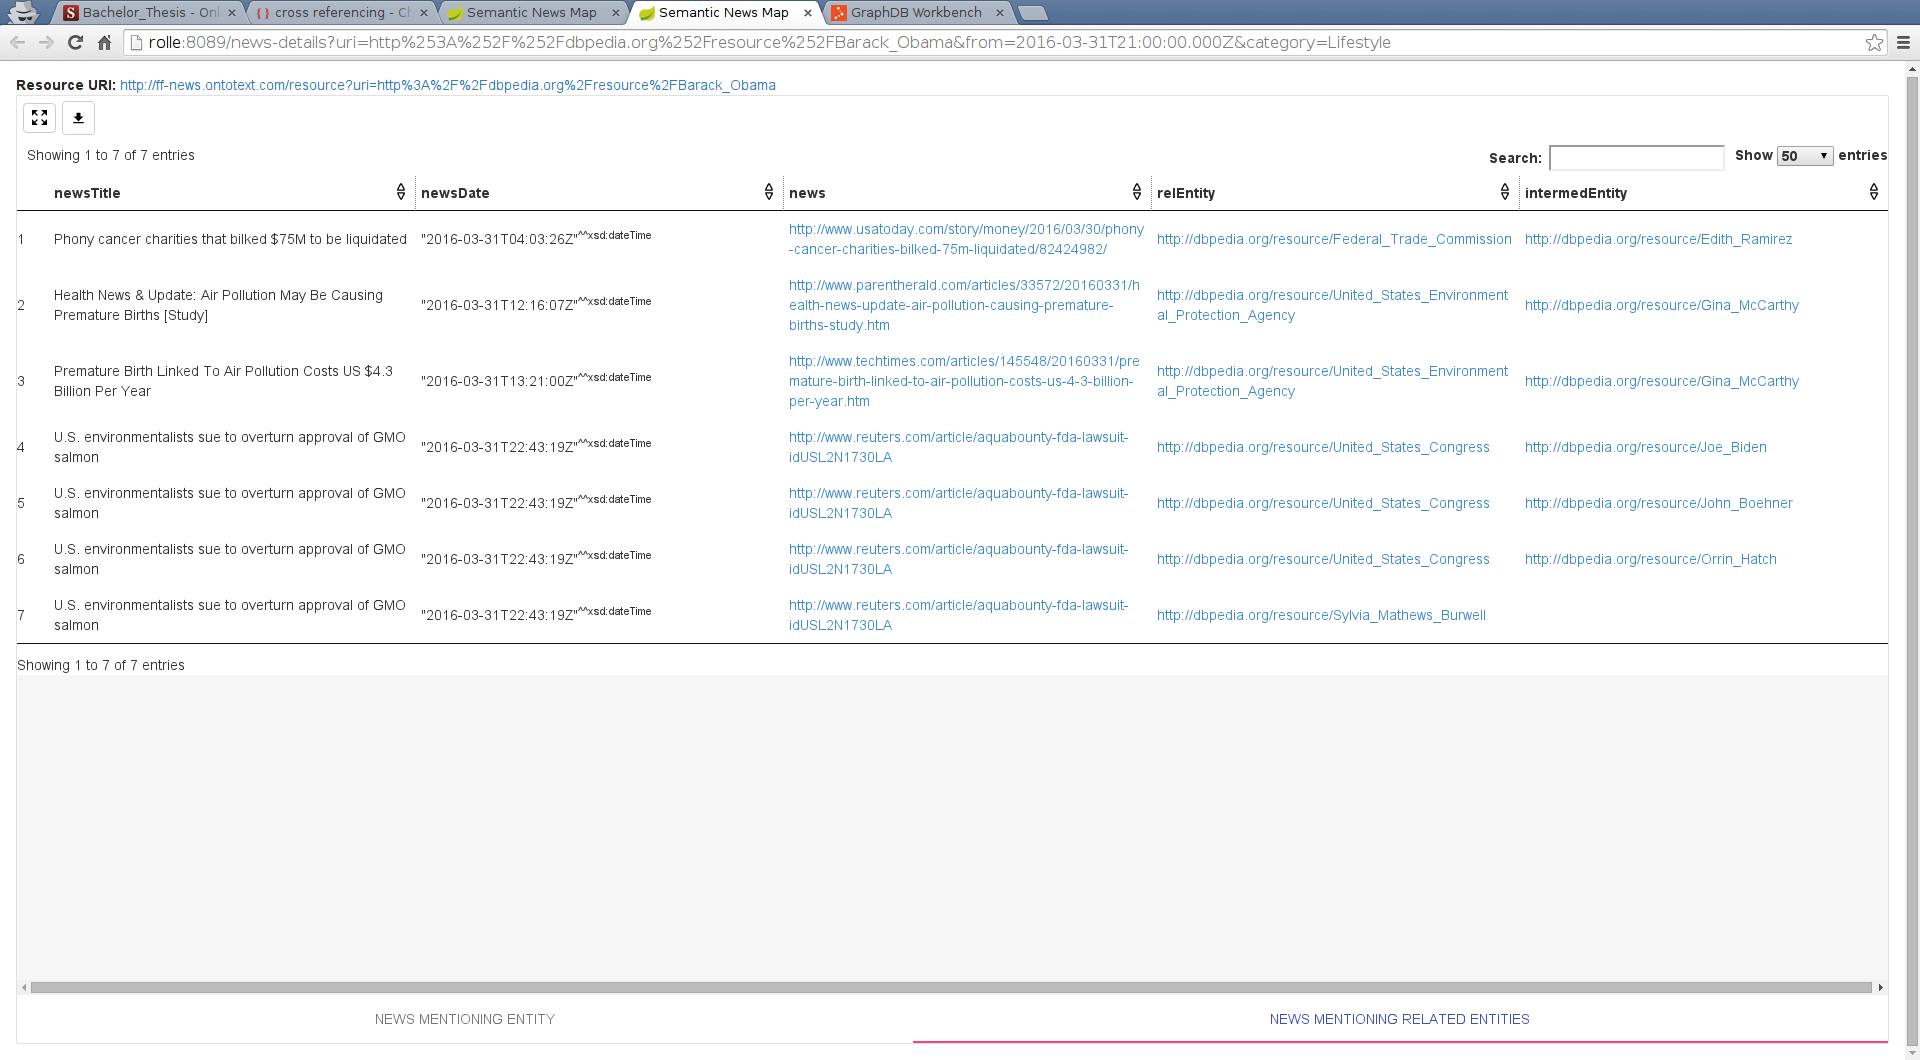
\includegraphics[width=\linewidth]{news-mentioning-related-entities}
    \caption{News mentioning related entities view}
    \label{fig:news-mentioning-related-entities}
\end{figure}



\section{Architecture and used technologies}
The whole application is based on a classic \verb|Client-Server| architecture. There is a backend part and a frontend part. The entire project is managed by \verb|Apache Maven| - a build system for compiling, packaging and dependency management of Java-based projects. It uses the standard Maven project archetype and contains two modules:
\begin{verbatim}
    semantic-news-server
    semantic-news-ui
\end{verbatim}
The first is the backend module which contains only \verb|Java 8| code, connects to the FF-News GraphDB\textsuperscript{TM} repository and executes the news aggregation SPARQL queries which will feed the frontend of the application with data. And the second module is the frontend module which only contains \verb|Javascript|, \verb|HTML| and \verb|CSS| code but its build lifecycle is again managed by Maven.

Communication between both modules is accomplished via REST (Representational State Transfer) in order to assure total decoupling of both components so that they can be easily modified without affecting each other. A simple example could be the frontend making a HTTP request to:\\
\texttt{http://<url-host>/rest/semnews/news-mentioning-country?\\countryCode=USA\&from=2016-04-12}\\ and the backend sending a response containing the results from the execution of the SPARQL query about news titles and URLs of news from 12.April 2016, mentioning the United States in JSON format which the frontend can easily read and handle. 

\subsubsection{Semantic News Map Server (Backend)}
The backend part is written in \texttt{Java 8} using the \texttt{Spring Framework} as a web framework. More specifically \texttt{Spring Boot} is used, which makes it easy to create stand-alone, production-grade Spring based applications that are extremely easy to deploy. It includes an embedded \texttt{Apache Tomcat} application server which eliminates the need for exporting \texttt{.war} files, configuring a Tomcat instance separately, copying the \texttt{.war} file in the Tomcat distribution and launching the server. Spring Boot generates for you an executable \texttt{.jar} file with an already configured embedded application server which only needs to be executed and that is all.

\subsubsection{Semantic News Map UI (Frontend)}
The frontend part is entirely based on AngularJS Javascript MVC framework. AngularJS is a framework for building Single Page Applications (SPA). This means that the server only serves the \texttt{index.html} file on start which then loads all other needed libraries, stylesheets and templates. From there on Angular handles routing, rendering of different views and all other UI specific logic. It will need the backend only as a data provider through AJAX calls to it as was demonstrated above. This style of architecture is called \texttt{Client-Side MVC}.

All Javascript code in the project is written using the newest ECMAScript standard ES6 (ES2015) where there are now features like block-scoped variables with \texttt{let} instead of \texttt{var}, cleaned up syntax for object-oriented programming resembling more Java-style classes and a built-in module system with keywords such as \texttt{import}, \texttt{export} and \texttt{from}. But due to the fact that not all new features are implemented by all browsers, a transpiler called \texttt{Babel} is used which translates code written in ES6 to ES5. The module system at the time of writing this thesis is still not available in any browser yet, so a library called \texttt{SystemJS} is used which expands \texttt{import} statements to SystemJS calls in order to load needed resources.

Javascript dependency management is handled by \texttt{NPM (Node Package Manager)} from NodeJS and \texttt{JSPM}. JSPM is а package manager integrated with SystemJS module loader and works very well with ES6 code.

Most of the UI components are based on Google's design specification \textit{Material Design} used in Android Lollipop and above. AngularJS has an implementation of this spec called \texttt{Angular Material} which is used throughout the whole user interface.

All visualizations in the application are SVG-based and implemented with a library called \texttt{D3 (Data Driven Documents)}. Word clouds use an additional layout to the library called \texttt{d3-cloud} and the geographic heat map also uses an external layout called \texttt{d3-geomap}.
